% \documentclass{report}

% \usepackage{subcaption} % package for subfigures
% \usepackage{hyperref}  % package for linking figures etc
% \usepackage{enumitem}  % package for description with bullets
% \usepackage{graphicx}  % package for importing images
% \usepackage{mathtools} % package for math equation
% \usepackage{mathrsfs}  % package for math font
% \usepackage{indentfirst} % package for getting ident after section or paragraph
% \usepackage{multirow}  % package for tables, multirow
% \usepackage{longtable} % package for multi pages tables


% \usepackage[export]{adjustbox}
% % \usepackage{amsmath}

% \setlength{\parindent}{2em} % how much indent to use when we start a paragraph

% \graphicspath{ {./theory/figures/} }       % path for images

% \begin{document}

\chapter{Connecting Tubes}
\section{Introduction}
In the previous chapter, we described methods for generating candidate action tubes given a small video segment lasting 8 or 16 frames. However, actual videos
and actual human actions, in the  wild, last more than 16 frames most of the times. Current networks are unable to process a whole video at once, in order to generate action tubes
due to memory and computing power issues.  As mentioned in chapter 2, a lot action localization approaches deal with this situation by giving a video either
propose candidate areas in the frame-level and then they connect these in order to generate action tube proposal either, separate it into video segments,
proposing  sequences of bounding boxes for each video segment and then link them in order to generate action proposals. Both aforementioned techniques make
the suitable choice of linking method an important factor for the performance of the network. That's because, even though frame-level or video segment-level proposals
might be very good, if the proposed connection algorithm doesn't work well, final action tube proposals won't be efficient, so the final model will never
be able to achieve high classification performance. In other words, if connecting algorithm doesn't generate action proposals with great recall and MABO performance,
the model's classifier won't be able to perform suitable classification, because probably it would be given action tubes without any context.
In this chapter, we present 3 different approaches used for linking proposed ToIs generated from TPN in the previous chapter.

\section{First approach: combine overlap and actioness}
Our algorithm is inspired by \cite{DBLP:journals/corr/HouCS17}, which calculates all possible sequences of ToIs. In order find the best candidate action tubes,
it uses a score, which tells us how likely a sequence of TOIs is  to contain an action. This score is a combination of 2 metrics:
\begin{description}
\item[ Actioness,  ] which is the TOI's possibility to contain an action. This score is produced by TPN's scoring layers.
\item [ TOIs' overlapping, ] which is the IoU of the last bounding boxes of the first TOI and the first frames of the second TOI.
\end{description}

The above scoring policy can be described by the following formula:
\[ S = \frac{1}{m} \sum_ {i=1}^{m} Actioness_i + \frac{1}{m-1} \sum_{j=1}^{m-1} Overlap_{j,j+1} \]

For every possible combination of TOIs we calculate their score as show in figure \ref{fig:connection_algo}.

\begin{figure}[h]
  \centering
  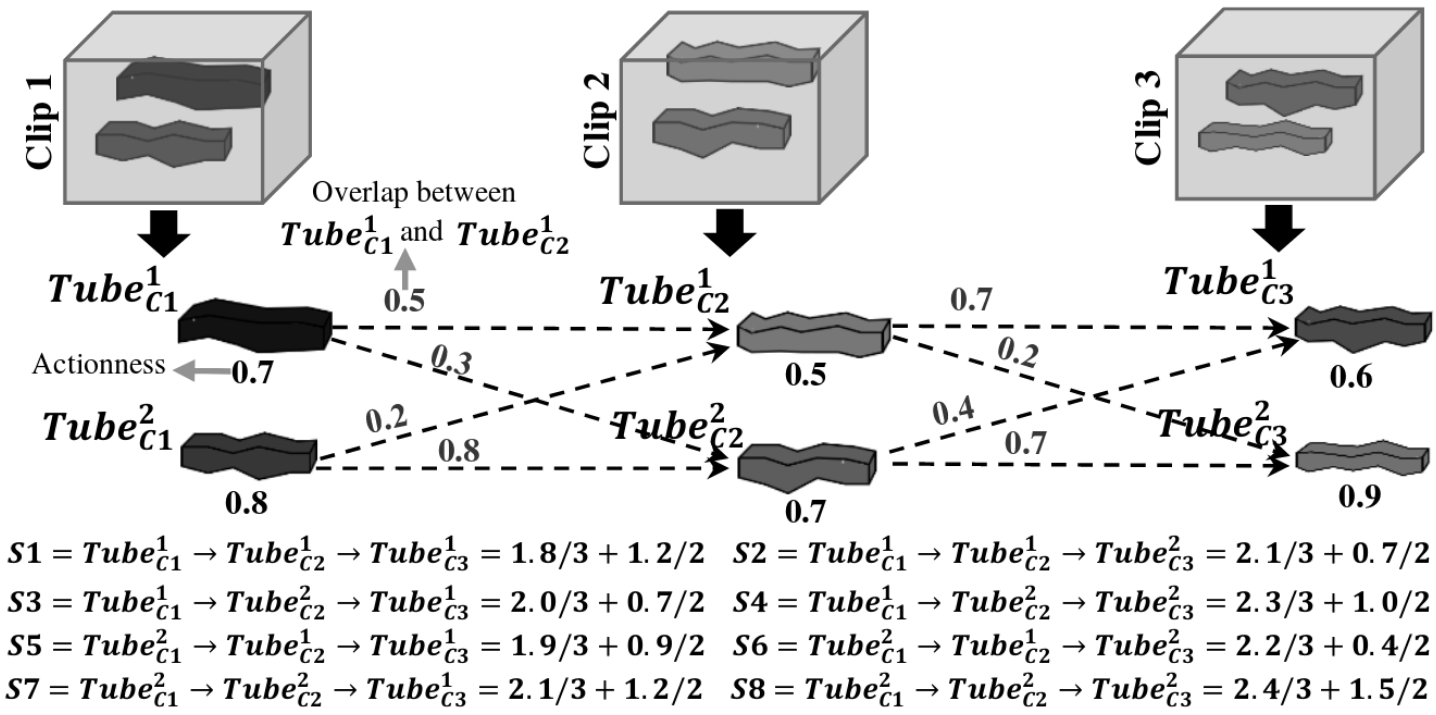
\includegraphics[scale=0.225]{connection_algo}
  \caption{An example of calculating connection score for 3 random TOIs taken from \cite{DBLP:journals/corr/HouCS17}}
  \label{fig:connection_algo}
\end{figure}

The above approach, however, needs too much memory for all needed calculations, so a memory usage  problem is
appeared. The reason is, for every new video segment, we propose \textit{k TOIs} (16 during training and 150 during validation).
As a result, for a small video separated into  \textbf{10 segments}, we need to calculate 
\textbf{  150\textsuperscript{10} scores} during validation stage. This causes our system to overload and it takes too much time to process
just one video. \par

In order to deal with this problem, we create a greedy algorithm in order to find the candidates tubes. Intuitively, this algorithm after
getting  a new video segment, keeps tubes with a score higher than a threshold, and deletes the rest. So, we don't need to calculate combinations with a
very low score. We wrote code for calculating tubes' scores in CUDA language, which has the ability to
parallel process the same code using different data. Our algorithm is described below:

\begin{enumerate}
\item Firstly,  initialize empty lists for the final tubes, final tubes' duration, their scores, active tubes, their corresponding duration,
  active tubes' overlapping sum and actioness sum where:
  \begin{itemize}
  \item Final tubes list contains all tubes which are the most likely to contain an action, and their score list contains their
    corresponding scores. We refer to each tube by its index, which is related a tensor, in which we saved all the ToIs proposed
    from TPN for each video segment.
  \item Active tubes list contains all tubes that will be matched with the new TOIs. Their overlapping sum list and actioness sum list
    contain their sums in order to avoid calculating then for each loop. 
  \end{itemize}
Also, we initialize  connection threshold equal to 0.5 .
\item For the first video segment, we add all the TOIs to both active tubes and final tubes. Their scores are only their actioness because
  there are no tubes for calculating their overlapping score. So, we set their overlaping sum equal to 0.
\item For each next video, after getting the proposed ToIs, firstly we calculate their overlapping score with each active tube. Then, we
  empty active tubes, active tubes' duration, overlapping sum and actioness score lists.  For each new tube that has a score higher than the
  connection threshold,  we add both to final tubes and to active tubes and their corresponding lists, and we increase their duration.
\item If the number of active tubes is higher than a threshold, we set connection threshold equal to the score of
  the 100th higher score. On top of that, we update the final tubes list, removing all tubes that have score lower than the threshold.
\item After that, we add in active tubes, the current video segment's proposed TOIs, alongside with their actioness scores in the  actioness sum list and
  zero values in corresponding positions in the overlaps sum list (such as in the 1st step).
\item We repeat the previous 3 steps until there is no video segment left.
\item Finally, as we mentioned before, we have a list which contains the indexes of the saved tubes. So, we modify them in order to have
  the corresponding bounding boxes. However, 2 succeeding ToIs do not, always, have exactly the same bounding boxes in the frames that overlap. For example,
  ToIs from the $1^{st}$ video segment start from frame 1 to frame 16. If we have video step equal to 8, these ToIs overlap temporally
  with the ToIs from the  succeeding video segment in frames 8-16. In those frames, in final tube, we choose the area that contains both bounding boxes which is
  denoted as $(min(x_1,x'_1), min(y_1,y'_1), max(x_2,x'_2), max(y_2,y'_2))$ for bounding boxes $(x_1,y_1,x_2,y_2)$ and $(x'_1,y'_1,x'_2,y'_2)$.
\end{enumerate}
% We implement this algorithm using CUDA language for counting the scores. In \cite{DBLP:journals/corr/HouCS17}, they use temporal \textit{stride = sample duration} during testing. We want 
\subsection{JHMDB Dataset}

In order to validate our algorithm, we firstly experiment in JHMDB dataset's videos in order to define the best overlapping policy and
the video overlapping step. Again, we use recall as evaluation metric. A groundtruth action tube is considered to be found, as well as positive,
if there is at least 1 video tube which overlaps with it over a predefined threshold, otherwise it .  These thresholds are again 0.5, 0.4 and 0.3.
We set TPN to return 30 ToIs per video segment.
We chose to update threshold when active tubes are more than 500 and to keep the first 100 tubes as active. We did so, because, a big part of the
code is performing in the CPU. That's because, we use lists, which are very easy to handle for adding and removing elements. So, if we use bigger update
limits, it takes much more time to process them.

\paragraph{Sample duration equal to 16 frames} At first we use as sample duration = 16 and video step = 8. As overlapping frames we count frames
\textit{(8...15)} so we have \#8 frames. Also, we use only \#4 frames with combinations \textit{(8...11), (10...13) and (12...15)} and 
\#2 frames with combinations \textit{(8,9), (10,11), (12,13), and (14,15)}. The results are shown in Table \ref{table:step8_16} (in bold are
the frames with which we calculate the overlap score).

\newpage
\begin{center}
\begin{longtable}{||c||c c c||}

  \hline
  \multirow{2}{5em}{combination} & {} &overlap thresh & {} \\
                                    &  0.5  &  0.4 &  0.3 \\         
  \hline  \hline
  0,1,...,\textbf{\{8,...,15\}}               & {} & {} & {} \\
  \textbf{\{8,9,...,15\}},16,...,23           & 0.3172 & 0.4142 & 0.6418 \\
  \hline     \hline                          


  0,1,...,\textbf{\{8,...,11,\}}...,14,15     & {} & {} & {} \\
  \textbf{\{8,...,11\}},12,...,22,23          & 0.3172 & 0.4142& 0.6381 \\
  \hline
  0,1,...,\textbf{\{10,...,13,\}}14,15,       & {} & {} & {} \\
  8,9,\textbf{\{10,...,13\}},14,...,22,23     & 0.3209 &0.4179   & 0.6418 \\
  \hline
  0,1,...,\textbf{\{12,...,15,\}}             & {} & {} & {} \\
  8,9,...,\textbf{\{12,...,15\}},16,...,23,   & 0.3284 & 0.4216 & 0.6381 \\
  \hline     \hline                          

  0,1,...,\textbf{\{8,...,11,\}},...,14,15,   & {} & {} & {} \\
  \textbf{\{8,9,...,11,\}}12,...,22,23        & 0.3172   & 0.4142& 0.6381 \\
  \hline
  0,1,...,\textbf{\{10,...,13,\}}14,15,       & {} & {} & {} \\
  \textbf{\{10,...,13\}},14,...,22,23         & 0.3209 &0.4179   & 0.6418 \\
  \hline
  0,1,...,\textbf{\{12,...,15\}}              & {} & {} & {} \\
  8,9,...,\textbf{\{12,...,15\}},16,...       & 0.3284 & 0.4216 & 0.6381 \\
  \hline \hline
  
  0,1,...,\textbf{\{8,9,\}},10,...,14,15,     & {} & {} & {} \\
  \textbf{\{8,9,\}}10,11,...,22,23            & 0.3134   & 0.4104 & 0.6381 \\
  \hline
  0,1,...,\textbf{\{10,11,\}},12,...,14,15,   & {} & {} & {} \\
  8,9,\textbf{\{10,11,\}}12,...,22,23         & 0.3209   & 0.4216 & 0.6418 \\
  \hline
  0,1,...,\textbf{\{12,13,\}},14,15,          & {} & {} & {} \\
  8,9,...,\textbf{\{12,13,\}}14,...,22,23     & 0.3246   & 0.4179 & 0.6418 \\
  \hline
  0,1,...,13,\textbf{\{14,15,\}}              & {} & {} & {} \\
  8,9,...,\textbf{\{14,15,\}}16,...,22,23     & 0.3321   & 0.4216 & 0.6306 \\
  \hline \hline
  \caption{Recall results for step = 8}
  \label{table:step8_16}
\end{longtable} 
\end{center}

As we can from the above table, generally we get very bad performance and we got the best performance when we calculate the overlap between only 2 frames (either \textit{14,15} or \textit{12,13}).
So, we thought that we should increase the video step because, probably, the connection algorithm is too strict into big movement variations during  the video. As a result, we set video step = 12 which
means that we have only 4 frames overlap. In this case,  for \#4 frames, we only have the combination \textit{(12...15)}, for \#2 frames we have \textit{(12,13), (13,14) and (14,15)} as shown in
Table \ref{table:step12_16}.

\begin{center}
\begin{longtable}{||c||c c c||}

  \hline
  \multirow{2}{5em}{combination} & {} &overlap thresh & {} \\
                                    &  0.5  &  0.4 &  0.3 \\         
  \hline  \hline
  0,1,...,11,\textbf{\{12,...,15\}}           & {} & {} & {} \\
  \textbf{\{12,13,...,15\}},16,...,26,27         & 0.3769 & 0.4627 & 0.6828 \\
  \hline     \hline                          

  0,1,...,\textbf{\{12,13,\}},14,15,          & {} & {} & {} \\
  \textbf{\{12,13,\}}14,15,...,26,27          & 0.3694   & 0.4627 & 0.6903 \\
  \hline                          
  0,1,...,12\textbf{\{13,14,\}},15,           & {} & {} & {} \\
  12,\textbf{\{13,14,\}}15,...,26,27          & 0.3843   & 0.4627 & 0.6828 \\
  \hline                          
  0,1,...,12,13\textbf{\{14,15,\}}            & {} & {} & {} \\
  12,13,\textbf{\{14,15,\}}16,...,26,27       & 0.3694   & 0.459 & 0.6828 \\
  \hline     \hline                          

  \caption{Recall results for step = 12}
  \label{table:step12_16}
\end{longtable} 
\end{center}

As we can see, recall performance is increased so that means that our assumption was correct. So again, we increase video step into 14, 15 and 16 frames
and recall score is shown in Table \ref{table:step14_16}
\begin{center}
\begin{longtable}{||c||c c c||}

  \hline
  \multirow{2}{5em}{combination} & {} &overlap thresh & {} \\
                                    &  0.5  &  0.4 &  0.3 \\         
  \hline  \hline
  0,1,...,13\textbf{\{14,15\}}                & {} & {} & {} \\
  \textbf{\{14,15\}},16,...,28,29                & 0.3731 & 0.5336 & 0.6493 \\
  \hline     \hline                          

  0,1,...,13,\textbf{\{14,\}}15,              & {} & {} & {} \\
  \textbf{\{14,\}}15,...,28,29                & 0.3694   & 0.5299 & 0.6455 \\
  \hline                          
  0,1,...,14,\textbf{\{15\}}                  & {} & {} & {} \\
  14,\textbf{\{15,\}}16,...,28,29             & 0.3731   & 0.5187 & 0.6381 \\
  \hline  \hline

  0,1,...,14,\textbf{\{15\}}                & {} & {} & {} \\
  \textbf{\{15\}},16,...,30                 & 0.3918 & 0.5187 & 0.6381 \\
  \hline     \hline                          
  0,1,...,14,\textbf{\{15\}}                & {} & {} & {} \\
  \textbf{\{16\}},17,...,31                 & 0.4067 & 0.7313 & 0.8731 \\
  \hline                          
  \caption{Recall results for steps = 14, 15 and 16}
  \label{table:step14_16}
\end{longtable} 
\end{center}

The results show that we get the best recall performance when we have no overlapping steps and video step = 16 = sample duration. We try to improve
more our results, using smaller duration because, as we saw from TPN recall performance, we get better results when we have sample duration = 8 or 4.

\paragraph{Sample duration equal to  8}
We wanted to confirm that we get the best results, when we have no overlapping frames and step = sample duration. So Table \ref{table:step4_8}
shows recall performance for sample duration = 8 and video step = 4 and Table \ref{table:step8_678 } for video steps = 6, 7 and 8.


\begin{center}
\begin{longtable}{||c||c c c||}

  \hline
  \multirow{2}{5em}{combination} & {} &overlap thresh & {} \\
                                    &  0.5  &  0.4 &  0.3 \\         
  \hline  \hline
  0,1,2,3,13\textbf{\{4,5,6,7\}}                & {} & {} & {} \\
  \textbf{\{4,5,6,7\}},8,9,10,11                & 0.2015   & 0.3582 & 0.5858 \\
  \hline     \hline                          

  0,1,2,3,\textbf{\{4,5,\}}6,7                  & {} & {} & {} \\
  \textbf{\{4,5,\}}6,7,8,9,10,11                & 0.1978   & 0.3582 & 0.5933 \\
  \hline                          
  0,1,2,3,4\textbf{\{5,6,\}}7                   & {} & {} & {} \\
  4,\textbf{\{5,6,\}}7,8,9,10,11                & 0.1978   & 0.3507 & 0.5821 \\
  \hline                          
  0,1,2,3,4,5\textbf{\{6,7\}}                   & {} & {} & {} \\
  4,5,\textbf{\{6,7,\}}8,9,10,11                & 0.194   & 0.3433 & 0.585 \\
  \hline                           
  \caption{Recall results for step = 4}
  \label{table:step4_8}
\end{longtable} 
\end{center}

\begin{center}
\begin{longtable}{||c||c c c||}

  \hline
  \multirow{2}{5em}{combination} & {} &overlap thresh & {} \\
                                    &   0.5  &  0.4 &  0.3 \\         
  \hline  \hline
  0,1,2,3,4,5\textbf{\{6,7\}}           & {} & {} & {} \\
  \textbf{\{6,7\}},8,9,10,11,12,13      & 0.3134  & 0.7015 & 0.8619 \\
  \hline     \hline                          

  0,1,2,3,4,5,\textbf{\{6,\}}7          & {} & {} & {} \\
  \textbf{\{6,\}}7,8,9,10,11,12,13      & 0.3209  & 0.6679 & 0.847 \\
  \hline                          
  0,1,2,3,4,5,6,\textbf{\{7\}}          & {} & {} & {} \\
  6,\textbf{\{7\}}8,9,10,11,12,13       & 0.3172  & 0.6567 & 0.8507 \\
  \hline                          
  0,1,2,3,4,5,6\textbf{\{7\}}           & {} & {} & {} \\
  \textbf{\{7,\}}8,9,10,11,12,13,14     & 0.5597  & 0.7687 & 0.903 \\
  \hline                           
  0,1,2,3,4,5,6\textbf{\{7\}}           & {} & {} & {} \\
  \textbf{\{8\}}9,10,11,12,13,14,15     & 0.653	  & 0.8396 &0.9179  \\
  \hline                           
  \caption{Recall results for steps = 6, 7 and 8}
  \label{table:step8_678 }
\end{longtable} 
\end{center}

According to Tables \ref{table:step4_8} and \ref{table:step8_678 }, it is clearly shown that, we achieve the  best results, for $step = sample duration$ and overlapping scores is calculated between the last box of the current tubes and the first box of next tubes.

\subsection{UCF dataset}
In previous steps, we tried to find the best overlap policy for our algorithm in JHMDB dataset. After that, it's time to apply our algorithm in UCF dataset using the best scoring
overlap policy. We did some modifications in the code, in order to use less memory and we moved most parts of the code to the GPU. This happened by using tensors instead of lists for scores while
most operations are, from now on, matrix operations. On top that, the last step of the algorithm, which is the modification from indices to actual action tubes is written, now, in CUDA code so
it takes place in the GPU, too. So, we are now able to increase the number of ToIs returned by TPN, the max number of active tubes before updating threshold and the max number of final
tubes. \par
The first experiments we performed were related to the number of the final tubes, our network proposes alongside with TPN's proposed
tubes' number. We experiment for cases, in which TPN proposes 30, 100 and 150 ToIs, our final network proposes 500, 2000 and 4000
candidate action tubes for sample durations equal to 8 and 16 frames.
For the sample duration equal to 8 we return 100 ToIs because, when we tried to return 150 proposed ToIs, we got OutOfMemory error.
Table \ref{table:ucf_recall} show the spatiotemporal recall and MABO performance of those approaches. Furthermore, Table \ref{table:ucf_temp_recall } show their temporal recall and MABO performance. We are interested in temporal performance, because UCF consists of
untrimmed videos, unlike JHMDB which has only trimmed videos. So, we want to know how well our network is able to propose action tubes that
overlap temporally with the groundtruth action tubes over a ``big'' threshold. For temporal localization, we don't use 0.5, 0.4 and 0.3
overlapping threshold, but instead, we use 0.9, 0.8 and 0.7, because it is very important our network to be able to propose tubes that
 contain an action, at least from the temporal perspective. In order to calculate the temporal overlap, we use IoU for 1 dimension as described before.

\begin{center}
\begin{longtable}{||c | c | c ||c c c | c|}

  \hline
  \multirow{2}{*}{combination} & \multirow{2}{2.5em}{TPN tubes} & \multirow{2}{2.5em}{Final tubes} &  \multicolumn{3}{}{overlap thresh} & \multirow{2}{*}{MABO} \\
  {} & {} & {} &  0.5 &  0.4 & 0.3 & {}\\         
  \hline
  
  \multirow{6}{7em}{0,1,...,6,\textbf{\{7,\}}
  \textbf{\{8,\}}9,...,14,15 }  & \multirow{3}{*}{30} & 500   & 0.2829  & 0.4395 & 0.5817  & 0.3501 \\
  \cline{3-7}
  {} &  {}   & 2000   & 0.3567  & 0.4996 & 0.6289 & 0.3815\\
  \cline{3-7}
  {} &  {}   & 4000   & 0.3749  & 0.5316 & 0.6487 & 0.3934 \\
  \cline{2-7}
  {} &  \multirow{3}{*}{100}   & 500   & 0.2966  & 0.451 & 0.5947 & 0.356 \\
  \cline{3-7}
  {} &  {}   & 2000   & 0.3757  & 0.5163 & 0.6471 & 0.3902 \\
  \cline{3-7}
  {} &  {}   & 4000  & 0.3977  & 0.5506 & 0.6624 & 0.4029 \\
  \hline                                    
  \multirow{6}{7em}{0,1,...,14,\textbf{\{15,\}}
  \textbf{\{16,\}}17,18,...,23 }  & \multirow{3}{*}{30} & 500   & 0.362  & 0.5042 & 0.6243 & 0.3866 \\
  \cline{3-7}
  {} &  {}   & 2000   & 0.416  & 0.5468 & 0.6631 & 0.4108  \\
  \cline{3-7}
  {} &  {}   & 4000   & 0.4281  & 0.5589  & 0.6779 & 0.4182 \\
  \cline{2-7}
  {} &  \multirow{3}{*}{150}   & 500 & 0.3589  & 0.4981 & 0.6198 & 0.3845 \\
  \cline{3-7}
  {} &  {}   & 2000   & 0.4129  & 0.5392  & 0.6563 & 0.4085 \\
  \cline{3-7}
  {} &  {}   & 4000   & 0.4266  & 0.5521 & 0.6722 & 0.4162\\
  \hline                                    

  \caption{Recall results for UCF dataset}
  \label{table:ucf_recall}
\end{longtable} 
\end{center}

\begin{center}
\begin{longtable}{||c | c | c ||c c c| c|}

% \begin{table}
%   \centering
%   \setlength{\tabcolsep}{4pt}
%   \begin{tabular}{||c | c | c ||c c c| c|}

  \hline
  \multirow{2}{*}{combination} & \multirow{2}{2.5em}{TPN tubes} & \multirow{2}{2.5em}{Final tubes} &  {} &overlap thresh & {} & \multirow{2}{*}{MABO} \\
  {} & {} & {} &  0.9 &  0.8 & 0.7 & {}\\         
  \hline
  
  
  \multirow{6}{7em}{0,1,...,6,\textbf{\{7,\}}
  \textbf{\{8,\}}9,...,15 }  & \multirow{3}{*}{30} & 500   & 0.4464  & 0.581 & 0.6844  & 0.7787 \\
  \cline{3-7}
  {} &  {}   & 2000   & 0.635  & 0.7665 & 0.8403 & 0.8693 \\
  \cline{3-7}
  {} &  {}   & 4000   & 0.7034  & 0.8228 & 0.8875 & 0.8973 \\
  \cline{2-7}
  {} &  \multirow{3}{*}{100}   & 500   & 0.454 & 0.5924 & 0.692 & 0.783 \\
  \cline{3-7}
  {} &  {}   & 2000   & 0.651 & 0.7696 & 0.8441 &0.8734 \\
  \cline{3-7}
  {} &  {}   & 4000   & 0.7209 &0.8312 & 0.8913 & 0.9026 \\

  \hline                                    
  \multirow{6}{7em}{0,1,...,14,\textbf{\{15,\}}
  \textbf{\{16,\}}17,18,...,23 }  & \multirow{3}{*}{30} & 500   & 0.6844 &0.8327 & 0.9027 & 0.8992 \\
  \cline{3-7}
                                    {} &  {}   & 2000   & 0.7475 & 0.8684 & 0.9217 & 0.9175 \\
  \cline{3-7}
                                    {} &  {}   & 4000   & 0.7567  & 0.8745  & 0.9255 & 0.9211 \\
  \cline{2-7}
                                    {} &  \multirow{3}{*}{150}   & 500   & 0.7498 &0.8707 &0.9171 & 0.9125 \\
  \cline{3-7}
                                    {} &  {}   & 2000   & 0.8243 & 0.911 & 0.9392 & 0.9342\\
  \cline{3-7}
                                    {} &  {}   & 4000   &  0.8403  & 0.9179 & 0.9437 & 0.9389\\
  \hline                                    
  % \end{tabular}
  \caption{Temporal Recall results for UCF dataset}
  \label{table:ucf_temp_recall }
% \end{table}
\end{longtable} 
\end{center}

According to Table \ref{table:ucf_recall}, we achieve better recall and MABO performance when we set sample duration equal to 16.
In all cases,  recall performance of simulations with sample duration equal to  16 outweight the corresponding with 8, with the difference
varying from 2\% to 8\%. In addition, we get best recall and MABO performance when our system proposes 4000 tubes. As we can see,
the ratio of good proposals increases about 5\%-7\% when we change number of proposed tubes from 500 to 2000. This ratio increases more
when we double returned action tubes, from 2000 to 4000. However, this increase is only about 1\%-2\%, which make us rethink if this increase
is worth to be performed. That's because, this modification increases memory usage, because of 4000 proposed action tubes, instead of
2000. Finally, Table \ref{table:ucf_recall} shows that, for sample duration = 8, changing the number of ToIs produced by TPN, slightly
helps our network to achieve better results. This contribution is measured about 1\%-2\%.
On the contrary, when we set sample duration equal to 16, it slightly reduces network's performance. Taking all the aforementioned
results into account, we think that the most suitable choices for connection approaches are, for the sample duration equal to 8, the one in
which TPN returns 100 ToIs and our network proposes 4000 action tubes, and for the sample duration equal to 16, the one in which,
TPN returns 30 ToIs and the network 4000 action tubes. \par
Additionally, Table \ref{table:ucf_temp_recall } shows some interesting facts, too. At first, it confirms that increasing the number of proposed
action tubes, from 500 to 4000, increases recall and MABO performance. Also, we get better results when network has 16 frames as sample
duration, too. However, unlike Table \ref{table:ucf_recall}, Table \ref{table:ucf_temp_recall } shows that when we increase TPN's number
of proposed ToIs, it increases performances for both sample durations. For sample duration equal to 8, this increase results in improving
recall performances by 2\% and MABO performance by 1\% like spatiotemporal recall and MABO. For the sample duration equal to 16, recall
performance is increasing by about 8\% and MABO by 1\%-2\%.  \par
Taking both tables into consideration, we think that the best approach is TPN returning 30 proposed ToIs, network returning 4000 proposed
action tubes and sample duration equals with 16. We didn't choose TPN returning 150 proposed ToIs because, based on MABO performances,
they different only by 1\%, difference which is insignificant.


\subsubsection{Adding NMS algorithm}

Previous section describes the performances of network's proposals for variations in the number of  TPN's  returned ToIs, number of returned
proposed action tubes and sample duration. For each situation, we choose the k-best scoring action tubes, without taking into account
any relation between these action tubes, like their spatiotemporal overlap. So, like TPN's approach, we thought that we should apply
nms algorithm before choosing k-best scoring tubes, in order to further improve  spatiotemporal and temporal, recall and MABO  performance.
We experiment using again two sample durations, 16 and 8 frames per video segment, number or TPN's returning tubes equal to 30 and the
number of final picked action tubes equal to 4000. NMS algorithm uses a threshold in order to choose if 2 action tubes overlap enough. We
experiment setting this threshold equal to 0.7 and 0.8 and  the results are shown in Table \ref{table:ucf_nms_recall} for Spatiotemporal
performance and at Table \ref{table:ucf_nms_temp_recall} for temporal performance.

\begin{center}
  \setlength{\tabcolsep}{2pt}
\begin{longtable}{||c | c | c | c c c| c|}

  \hline
  \multirow{2}{*}{combination} & \multirow{2}{2.5em}{NMS thresh} & \multirow{2}{3.5em}{PreNMS tubes} &  {} &overlap thresh & {} & \multirow{2}{*}{MABO} \\
  {} & {} & {} &  0.5 &  0.4 & 0.3 & {}\\         
  \hline
  \multirow{3}{7em}{0,1,...,6,\textbf{\{7,\}}
  \textbf{\{8,\}}9,...,15 }  & 0.7 &\multirow{3}{*}{20000}  & 0.346 & 0.5202 & 0.657 & 0.3824685269 \\
  \cline{2-2} \cline{4-7} 
  {} &  0.8   & {}   & 0.3643 & 0.5392 & 0.6578 & 0.3904727407 \\
  \cline{2-2} \cline{4-7} 
  {} &  0.9   & {}   & 0.397  & 0.5574 & 0.6677 & 0.4031543642 \\
  \hline                                    
  \multirow{3}{7em}{0,1,...,14,\textbf{\{15,\}}
  \textbf{\{16,\}}17,...,23 }  & 0.7 & \multirow{3}{*}{20000}   & 0.3939 & 0.5559  & 0.6882 & 0.404689056 \\
  \cline{2-2} \cline{4-7} 
                                    {} &  0.8   & {}   & 0.4259 & 0.5764 & 0.6981 & 0.419487652 \\
  \cline{2-2} \cline{4-7} 
                                    {} &  0.9   & {}   & 0.4494 & 0.5856 & 0.7019 & 0.4302611039 \\

  \hline                                    

  \caption{Spatiotemporal Recall results for UCF dataset}
  \label{table:ucf_nms_recall}
\end{longtable} 
\end{center}

\newpage
\begin{center}
  \setlength{\tabcolsep}{2.2pt}
\begin{longtable}{||c | c | c | c c c| c|}

  \hline
  \multirow{2}{*}{combination} & \multirow{2}{2.5em}{NMS thresh} & \multirow{2}{3.5em}{PreNMS tubes} &  {} &overlap thresh & {} & \multirow{2}{*}{MABO} \\
  {} & {} & {} &  0.9 &  0.8 & 0.7 & {}\\         
  \hline
  \multirow{3}{7em}{0,1,...,6,\textbf{\{7,\}}
  \textbf{\{8,\}}9,...,15 }  & 0.7 &\multirow{3}{*}{20000}  & 0.6281 & 0.8251 & 0.9027 & 0.8885141223  \\
  \cline{2-2} \cline{4-7} 
  {} &  0.8   & {}   & 0.7369 & 0.8616 & 0.9148 & 0.9106069806 \\
  \cline{2-2} \cline{4-7} 
  {} &  0.9   & {}   &  0.7787 & 0.8753 & 0.9209 & 0.9212593589 \\
  \hline                                    
  \multirow{3}{7em}{0,1,...,14,\textbf{\{15,\}}
  \textbf{\{16,\}}17,...,23 }  & 0.7 & \multirow{3}{*}{20000}   & 0.7452 & 0.8920 & 0.9361 & 0.920331595 \\
  \cline{2-2} \cline{4-7} 
  {} &  0.8   & {}   & 0.8160 & 0.9278 & 0.9506 & 0.93612757 \\
  \cline{2-2} \cline{4-7} 
  {} &  0.9   & {}   & 0.854 & 0.9346 & 0.9529 & 0.9434986107 \\
  \hline                                    

  \caption{Temporal Recall results for UCF dataset}
  \label{table:ucf_nms_temp_recall}
\end{longtable} 
\end{center}

Comparing Table \ref{table:ucf_nms_recall} with Table \ref{table:ucf_recall},  we notice that NMS algorithm improves recall and MABO
performance when NMS threshold is equal to 0.9. When we set it equal to 0.7 or 0.8, we get worse results. This happens, probably, because
nms algorithm removes some good proposals. Comparing these results with results presented at Tables \ref{table:ucf_recall} and \ref{table:ucf_temp_recall } it becomes clear that using NMS algorithm is very useful. That's because, even though we get the same number of proposed action tubes,
these tubes are not very close spatiotemporally, so this makes proposed action tubes more likely to contain actual foreground action tubes.

\subsubsection{Stop updating threshold}

In previous approaches, scoring threshold was updated each time our algorithm gathered a significant number of ``active'' tubes in order not
to add action tubes with score below this score. However, after serious consideration, we came to the conclusion that sometimes, the updated
threshold leads to not detecting action tubes that start after some frames. That's because, until then, linking threshold may be too big that
won't let new action tubes to be created. So, we came with the modification of not updating linking threshold, but just filtering proposed
tubes, by keeping k-best scoring each time their number is bigger that the a specific number. The rest algorithm remains the same. Tables
\ref{table:ucf_nms_noup_recall} and \ref{table:ucf_nms_noup_temp_recall} show spatiotemporal and temporal, recall and MABO performance respectively.
We experiment for cases in which either we don't use the  NMS algorithm at all, either we set overlap threshold equal to 0.7 and 0.9 as shown
below.

\begin{center}
  \setlength{\tabcolsep}{2pt}
\begin{longtable}{||c | c | c | c c c| c|}

  \hline
  \multirow{2}{*}{combination} & \multirow{2}{2.5em}{NMS thresh} & \multirow{2}{3.5em}{PreNMS tubes} &  {} &overlap thresh & {} & \multirow{2}{*}{MABO} \\
  {} & {} & {} &  0.5 &  0.4 & 0.3 & {}\\         
  \hline
  \multirow{3}{7em}{0,1,...,6,\textbf{\{7,\}}
  \textbf{\{8,\}}9,...,15 }   &   \multicolumn{2}{|c|}{-}     &  0.3779 & 0.5316 & 0.6471 & 0.393082961 \\
  \cline{2-7}
  {} & 0.7 &\multirow{2}{*}{20000}  & 0.3483  & 0.5194 & 0.6471 & 0.3783524086 \\
  \cline{2-2} \cline{4-7} 
  {} &  0.9   & {}   & 0.416 & 0.5605 & 0.6722 & 0.4074053106 \\
  \hline                                    
  \multirow{3}{7em}{0,1,...,14,\textbf{\{15,\}}
  \textbf{\{16,\}}17,...,23 }  &   \multicolumn{2}{|c|}{-} & 0.438 & 0.5635 & 0.6829 & 0.4231788 \\
  \cline{2-7}
  {} & 0.7 & \multirow{2}{*}{20000}   & 0.4525 & 0.5848 & 0.7034 & 0.429747438 \\
  \cline{2-2} \cline{4-7} 
  {} &  0.9   & {}   & 0.3802 & 0.5133 & 0.6068 & 0.3862278851848662 \\

  \hline                                    

  \caption{Spatiotemporal Recall results for UCF dataset}
  \label{table:ucf_nms_noup_recall}
\end{longtable} 
\end{center}

\begin{center}
  \setlength{\tabcolsep}{2.2pt}
\begin{longtable}{||c | c | c | c c c| c|}

  \hline
  \multirow{2}{*}{combination} & \multirow{2}{2.5em}{NMS thresh} & \multirow{2}{3.5em}{PreNMS tubes} &  {} &overlap thresh & {} & \multirow{2}{*}{MABO} \\
  {} & {} & {} &  0.9 &  0.8 & 0.7 & {}\\         
  \hline

  \multirow{3}{7em}{0,1,...,6,\textbf{\{7,\}}
    \textbf{\{8,\}}9,...,15 }  &   -   & -    & 0.7087 & 0.8281 & 0.8913 & 0.899210587 \\
  \cline{2-7} 
  {} & 0.7 &\multirow{2}{*}{20000}  & 0.6586 & 0.854 & 0.9278 & 0.903373468 \\
  \cline{2-2} \cline{4-7} 
  {} &  0.9   & {}   &  0.8137 & 0.8973 & 0.9361 & 0.9333068498 \\
  \hline                                    
  \multirow{3}{7em}{0,1,...,14,\textbf{\{15,\}}
  \textbf{\{16,\}}17,...,23 }  &   \multicolumn{2}{|c|}{-} & 0.8327 & 0.9156 &0.9399 & 0.940143272 \\
  \cline{2-7}
  {} & 0.7 & \multirow{2}{*}{20000}& 0.8646 & 0.9369 & 0.9567 & 0.946701832 \\
  \cline{2-2} \cline{4-7} 
  {} &  0.9   & {}   & 0.6183 & 0.7696 & 0.8388 & 0.8628507037919737 \\
  \hline                                    

  \caption{Temporal Recall results for UCF dataset}
  \label{table:ucf_nms_noup_temp_recall}
\end{longtable} 
\end{center}

Comparing recall and MABO performances shown at Table \ref{table:ucf_nms_noup_recall} with those included in Tables \ref{table:ucf_nms_recall}
and \ref{table:ucf_recall}, we deduce that for the sample duration equal to 8, stopping updating linking threshold results in worse performance
when we set nms threshold equal to 0.7, but it achieves the best performances  when setting NMS threshold equal to 0.9 . Furthermore, for sample duration
equal to 16, we get, now,  best performance performance when we set nms threshold equal to 0.7 and worse performance for nms threshold equal to 0.9 .

\subsubsection{Soft-nms instead of nms}

After widely experiment using NMS algorithm, we thought that we should try to use Soft-NMS algorithm, introduced by \cite{DBLP:journals/corr/BodlaSCD17} and described in chapter 2. We implement our own soft-nms algorithm modifying it in order to calculate spatiotemporal overlapping
scores, and not just spatial, like the one implemented by \cite{DBLP:journals/corr/BodlaSCD17}. As mentioned before, instead of removing action tubes, Soft-NMS algorithm just reduces their score for those which overlap over a predefined threshol. We experiment for the sample duration
equal to 8 and thresholds equal to 0.7 and 0.9, because, our implementation ran out of memory for sample duration equal to 16.
Recall and MABO performance are presented in Tables \ref{table:ucf_softnms_recall} and \ref{table:ucf_softnms_temp_recall}

\begin{center}
  \setlength{\tabcolsep}{2pt}
\begin{longtable}{||c | c | c | c c c| c|}

  \hline
  \multirow{2}{*}{combination} & \multirow{2}{2.5em}{NMS thresh} & \multirow{2}{3.5em}{PreNMS tubes} &  {} &overlap thresh & {} & \multirow{2}{*}{MABO} \\
  {} & {} & {} &  0.9 &  0.8 & 0.7 & {}\\         
  \hline
  \multirow{2}{7em}{0,1,...,6,\textbf{\{7,\}}
  \textbf{\{8,\}}9,...,15 }  & 0.7 &\multirow{2}{*}{20000}  & 0.3916 & 0.5384 & 0.6464 & 0.3964639 \\
  \cline{2-2} \cline{4-7} 
  {} &  0.9   & {}   & 0.4023 & 0.5430 & 0.6502 & 0.398845313 \\
  \hline                                    

  \caption{Spatiotemporal Recall results for UCF dataset using Soft-NMS}
  \label{table:ucf_softnms_recall}
\end{longtable} 
\end{center}

\begin{center}
  \setlength{\tabcolsep}{2.2pt}
\begin{longtable}{||c | c | c | c c c| c|}

  \hline
  \multirow{2}{*}{combination} & \multirow{2}{2.5em}{NMS thresh} & \multirow{2}{3.5em}{PreNMS tubes} &  {} &overlap thresh & {} & \multirow{2}{*}{MABO} \\
  {} & {} & {} &  0.9 &  0.8 & 0.7 & {}\\         
  \hline

  \multirow{2}{7em}{0,1,...,6,\textbf{\{7,\}}
    \textbf{\{8,\}}9,...,15 }  & 0.7 &\multirow{2}{*}{20000}  & 0.7521 & 0.8586 & 0.9110 & 0.915746097  \\
  \cline{2-2} \cline{4-7} 
  {} &  0.9   & {}   & 0.7741 & 0.8768 & 0.9255 & 0.922677864 \\
  \hline                                    

  \caption{Temporal Recall results for UCF dataset using SoftNMS}
  \label{table:ucf_softnms_temp_recall}
\end{longtable} 
\end{center}

Taking results at Tables \ref{table:ucf_softnms_recall} and \ref{table:ucf_softnms_temp_recall} into consideration, alongside with those
at Tables \ref{table:ucf_nms_noup_recall} and \ref{table:ucf_nms_noup_temp_recall} for sample duration equal to 8, we notice that
using softNMS results in slightly better results. This happens when we set overlapping threshold equal to 0.9, otherwise, for
overlapping threshold 0.7, we get worst performance. Despite the fact that softnms results in better recall and MABO performance,
our implementation is very slow, which means that for a 201-frame video, softNMS part lasts about 32 seconds on the contrary with
standard NMS algorithm without updating linking threshold, in which this part last only 2 seconds. So, we choose to use the standard NMS
algorithm without updating liking threshold as an algorithm for  removing overlapping action tubes.

\section{Second approach: use progression and progress rate}
As we saw before, our first connecting algorithm doesn't have very good recall results. So, we created another algorithm which is based on
the one proposed by \cite{DBLP:journals/corr/abs-1903-00304}. This
algorithm introduces two new metrics according to \cite{DBLP:journals/corr/abs-1903-00304}:

% TODO add more description
\begin{description}
\item[ Progression,  ] which describes the probability of a specific action being performed in the TOI. 
  We add this factor because we have noticed that actioness is tolerant to false positives. Progression is
  mainly a rescoring mechanism for each class (as mentioned in \cite{DBLP:journals/corr/abs-1903-00304})

\item [ Progress rate, ] which is defined as the progress proportion that each action class has been performed.
  
\end{description}

So, each action tube is described as a set of TOIs
\[  T = {\{ {\bf t}_i^{(k)} | {\bf t}_i^{(k)} = ( t_i^{(k)}, s_i^{(k)}, r_i^{(k)} ) \}}_{i=1:n^{(k)},k=1:K} \]
where $ t_i^{(k)} $ contains TOI's spatiotemporal information, $ s_i^{(k)} $ its confidence score and $ r_i^{(k)} $ its progress rate.

In this approach, each class is handled separately, so for the rest section, we discuss action tube generation for one class only. In order to link 2 TOIs, for
a video with N video segments, the following steps are applied:
\begin{enumerate}
\item For the first video segment (k = 1), initialize an array with the M best scoring TOIs, which will be considered as active action tubes ( AT ).
  Correspondingly, initialize an array with M progress rates  and M confidence scores.
\item For k = 2:N, execute (a) to (c) steps:
  \begin{enumerate}
  \item Calculate overlaps between $ AT^{(k)} $ and $ TOIs^{(k)}. $
  \item Connect all tubes which satisfy the following criteria:
    \begin{enumerate}
    \item $ overlap score(at_i^{(k)},t_j^{(k)})   > \theta, 
      at  \in AT^{(k)}, t \in TOIs^{(k)}  $
    \item $r(at_i^{(k)}) < r(t_j^{(k)}) $ or 
      $r(t_i^{(k)}) - r(at_i{(k)}) < \lambda $
    \end{enumerate}
    
  \item For all new tubes update confidence score and progress rate as follows:
    \begin{description}
    \item The new confidence score is the average score of all connected TOIs:
      \[  s_z^{(k+1)} = \frac {1} {n} \sum_{n=0}^{k} s_i^{(n)}\]
    \item New progress rate is the highest progress rate:
      \[r(at_z^{(k+1)} = max(r(at_i^{(k)}), r(t_j^{(k)})) \]
    \end{description}
    % \item If $ progressrate(at_i^{(k)}) < progressrate(t_i^{(k)}) $ then $ progressrate(at_i^{(k+1)}) =
  \item Keep M best scoring action tubes as active tubes and keep K best scoring action tubes for classification.
  \end{enumerate}
  
\end{enumerate}

This approach has the advantage that we don't need to perform classification again because we already know the class of
each final tube. In order to validate our results, now, we calculate the recall only from the tubes which have the same
class as the groundtruth tube. Again, we considered a groundtruth  tube as positive if there is at least one proposed  tube
that overlaps with it over the predefined threshold

\begin{center}
\begin{longtable}{||c c||c c c||}
  \hline
  \multicolumn{2}{||c||}{\textbf{combination}} &\multicolumn{3}{|c||}{\textbf{overlap thresh}}\\

  \hline
  sample dur & step &   0.5  &  0.4 &  0.3 \\
  \hline   \hline
  8 & 6 & 0.3284 & 0.5 & 0.6082  \\
  \hline
  8 & 7 & 0.209	& 0.459 & 0.6119 \\
  \hline
  8 & 8 & 0.3060 & 0.5672 & 0.6866 \\
  \hline
  16 & 8  & 0.194 & 0.4366 & 0.7164 \\
  \hline
  16 & 12 & 0.3358 & 0.5336 & 0.7537 \\
  \hline
  16 & 16 & 0.2649 & 0.4664 & 0.709 \\
  
  \hline 

  \caption{Recall results for second approach with step = 8, 16 and their corresponding steps }
  \label{table:conn_app2}
\end{longtable} 
\end{center}

According to  Table \ref{table:conn_app2}, we get the best performance when we set sample duration equal to  16 and overlap step equal to 12.
Comparing this performance with the first approach, for both sample durations equal to 8 and 16, we notice that second approach falls short
comparing to the first one. 

\section{Third approach : use naive algorithm - only for JHMDB}

As mention in the first approach, \cite{DBLP:journals/corr/HouCS17} calculate all possible sequences of ToIs in order to the find the best
candidates. We rethought about this approach and we concluded that it could be implemented for JHMDB dataset if we reduce the number of proposed
ToIs, produced by TPN,  to 30 for each video clip. We exploited the fact that JHMDB dataset's videos are trimmed, so we do not need to look
for action tubes starting in the second video clip which saves us a lot of memory. On top of that, we modified our code
in order to be more memory efficient  writing some parts using CUDA programming language, saving a lot of processing power, too. \par
So, after computing all possible combinations starting of the first video clip and ending in the last video clip, we keep only the
\textbf{k-best scoring tubes (k = 500) }. We run experiments which have sample duration equal to 8 and 16 frames and we modify the video step each time.
For sample duration = 8, we return only 15 ToIs and for sample duration = 16, we return 30 because, if we return more, we get ``out of memory error''.
In the following table, we can see the recall results. \par  

\begin{center}
\begin{longtable}{||c c||c c c||}

  \hline
  \multicolumn{2}{||c||}{\textbf{combination}} &\multicolumn{3}{|c||}{\textbf{overlap thresh}}\\
  \hline
  sample dur & step &  0.5  &  0.4 &  0.3 \\
  \hline   \hline

  8 & 6 & 0.7873 & 0.8657 & 0.9366  \\
  \hline
  8 & 7 & 0.7836 & 0.8731 & 0.9366  \\
  \hline
  8 &  8 & 0.7910 & 0.8806 & 0.9515 \\
  \hline 

  16 & 8  & 0.7873 & 0.8843 & 0.9291 \\
  \hline
  16 & 12 & 0.7948 & 0.8881 & 0.9403 \\
  \hline
  16 & 16 & 0.7985 & 0.8918 & 0.9515 \\
  \hline 
  \caption{Recall results for third approach with  step = 8, 16 and their
corresponding steps}
  \label{table:conn_app3}
\end{longtable} 
\end{center}

From the above table, firstly, we confirm that when video step is equal to the sample duration gives us the best recall results.
Also, we notice that when sample duration is equal to 16  frames recall gets slightly better that when sample duration is
equal to 8. However, using  16 frames per video segment sample increases the memory usage even though it reduces the number of video segments, because of the
need to process bigger videos, bigger feature maps etc. So for the classification stage we will experiment using mostly sample duration equal
with 8 frames.

\section {General comments}

\begin{figure}[h]
  % 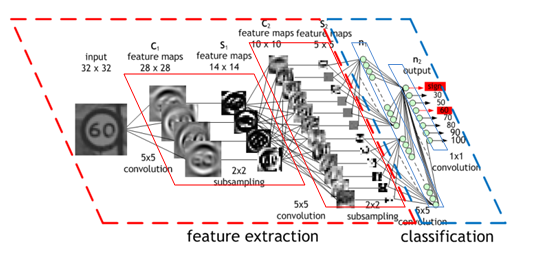
\includegraphics[scale=0.7]{convolutional_neural_network_structure} \]
  \centering
  % 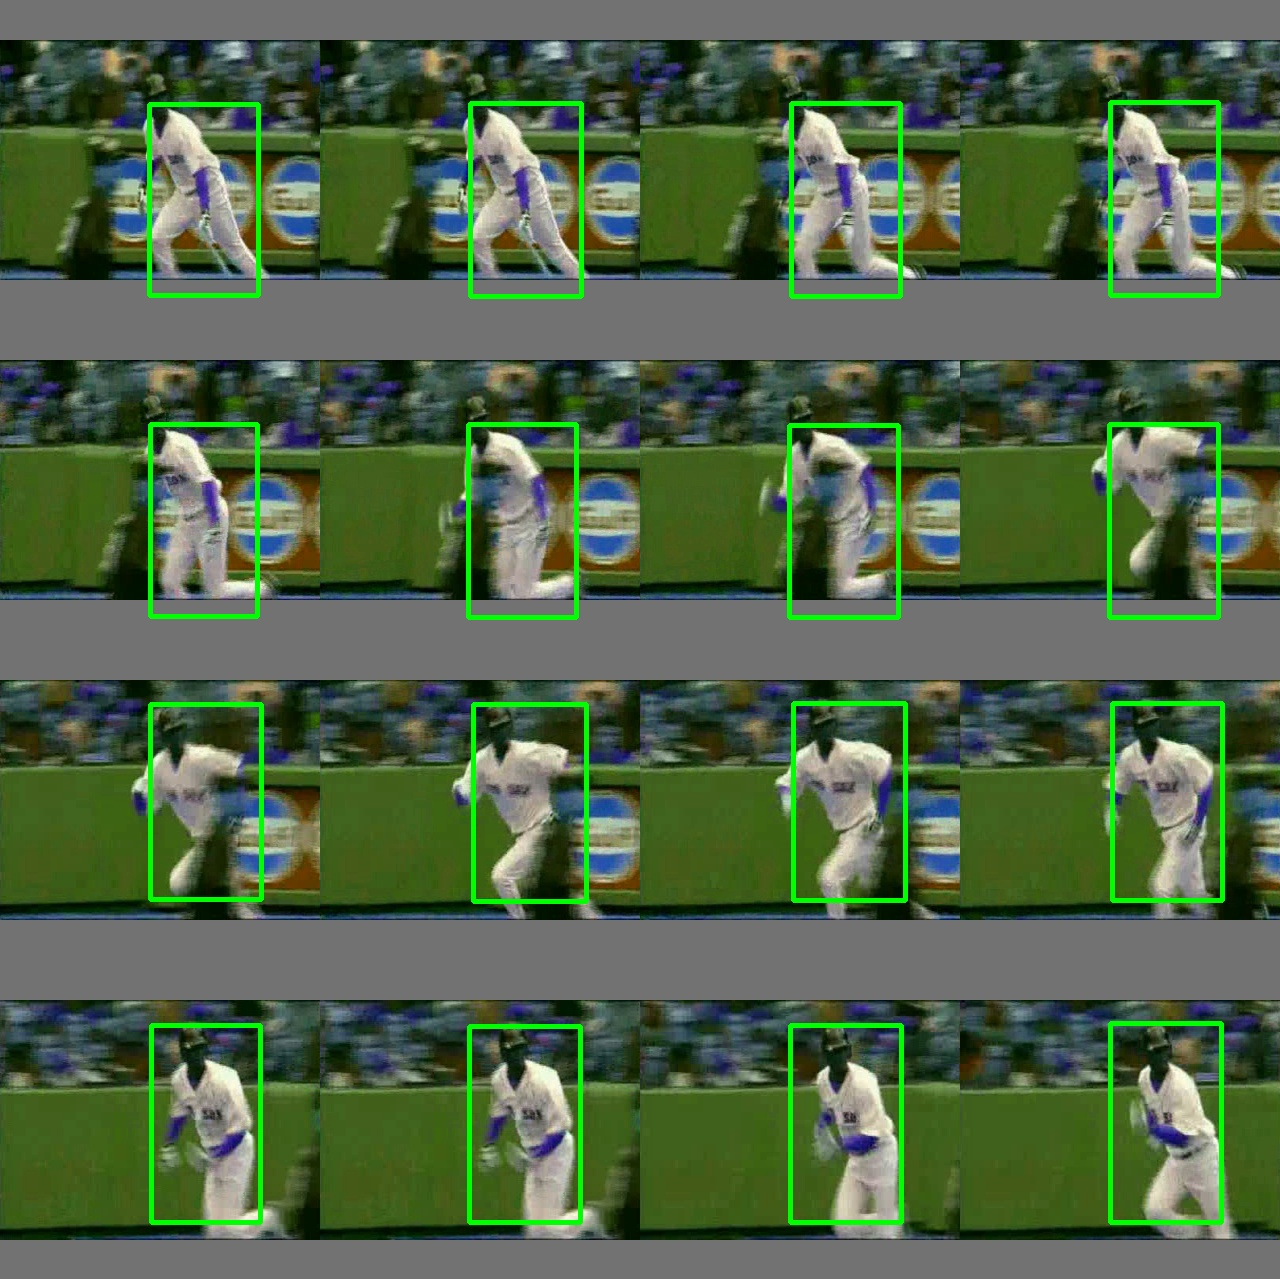
\includegraphics[scale=0.2]{tube_ex2_half}
  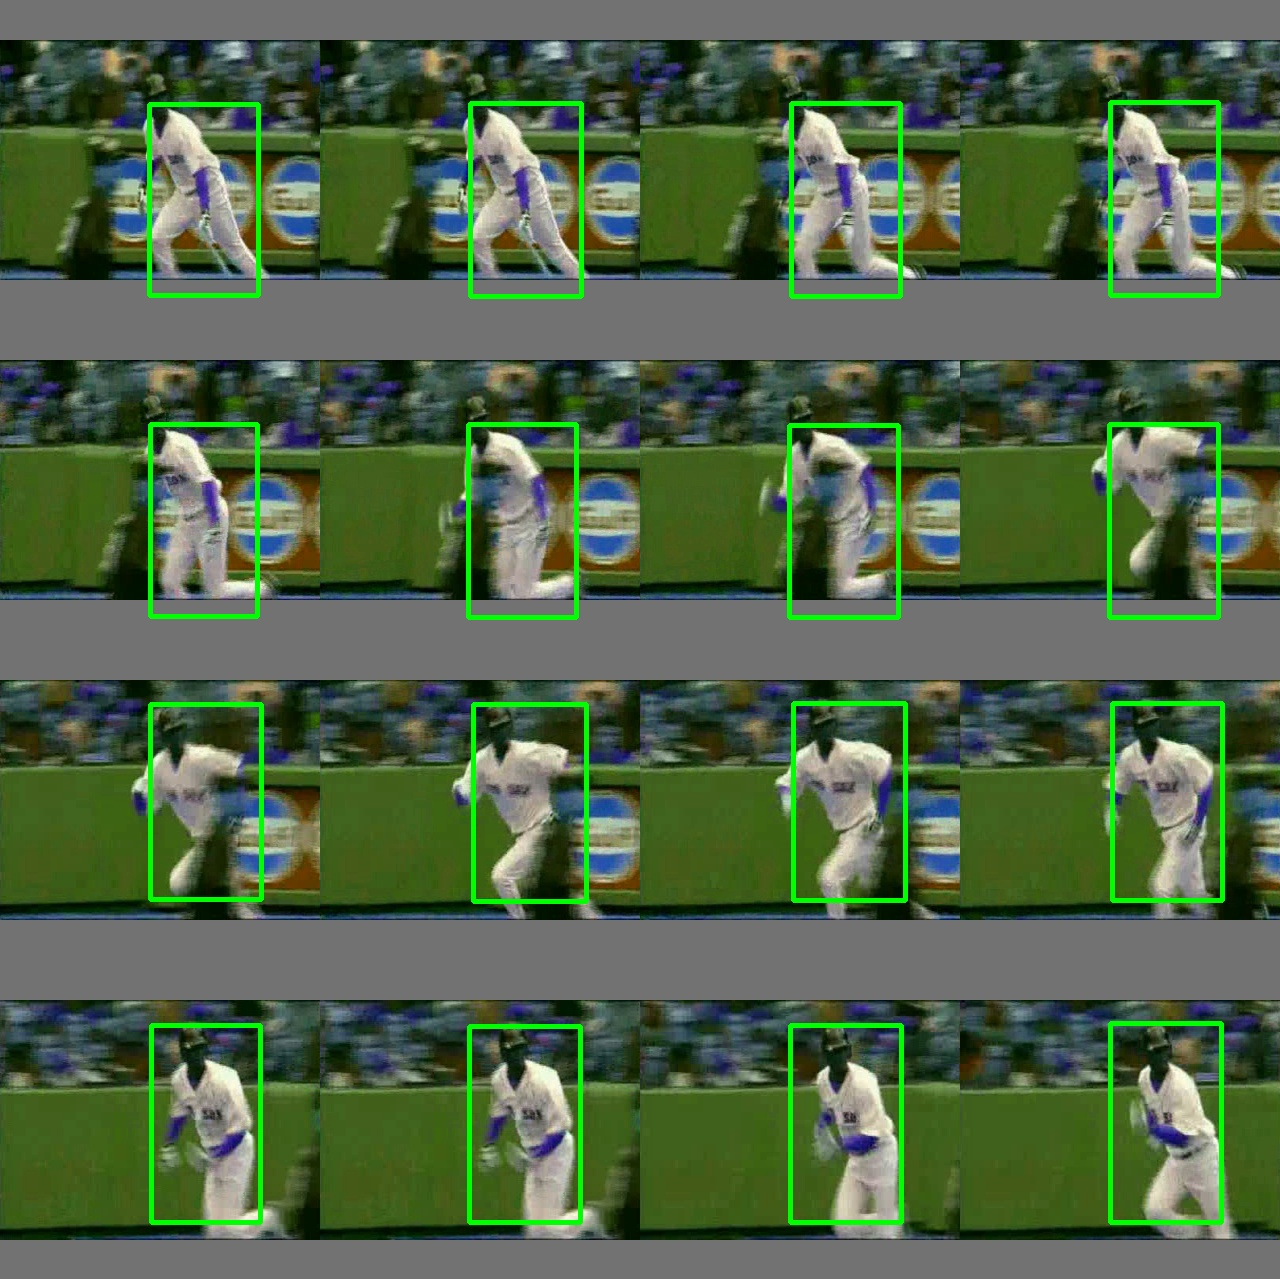
\includegraphics[width= 0.8\textwidth, height=0.45\textheight]{tube_ex2_half}
  \caption{Example of connected tubes}
  \label{fig:tube_ex}
\end{figure}

Figure \ref{fig:tube_ex} shows the example presented in chapter 3, after linking first video segment's first ToI with a ToI proposed for the second video segment. For this case, we used the third proposed method, including calculating all possible combinations. As shown in the Figure,
our algorithm manages to track the actor performing the action efficiently enough. This means that even though the actor moves during the
video, our approach manages not to loose contact with him. On top of that, it clear that the silhouette of the actor changes, and so does the area of proposed action tubes. The only problem which appears is that proposed action tubes sometimes exceeds the area of the actual video.
In order to deal with this problem, we set bounding boxes not to exceed these areas by keeping the limits of the original picture. So,
from now on, no bounding box will overlap with padding area.

% \end{document}
